
\documentclass[11pt,a4paper]{article}
\usepackage[margin=1in]{geometry}
\usepackage{amsmath,amssymb}
\usepackage{graphicx}
\usepackage{hyperref}
\usepackage{siunitx}

\title{Role Calculus: Band-Specific Coordination and Memory}
\author{}
\date{\today}

\begin{document}
\maketitle

\begin{abstract}
We introduce a minimal role calculus $(O,G,C,C^\ast)$ and testable physics anchors.
Test T2 establishes band-specific cross-coherence; Test T3 quantifies path dependence via hysteresis.
The suite is compact, falsifiable, and reproducible.
\end{abstract}

\section{Introduction}
% Short motivation, related work pointers (fill as needed).


% =====================
\section{Foundations}
\label{sec:foundations}

\subsection{Ur-Fabric and Roles}
We posit a minimal role calculus with observer $O$, generator $G$, counters $C$ and $C^\ast$, and a noise--structure axis $(N\!\leftrightarrow\!S)$ mediated by thresholds.
Here, $C$ counts fast, local events ("sparks"), while $C^\ast$ accumulates slow, integrated return channels ("glow").
This division is operational: $C$ is observable through short-window statistics; $C^\ast$ emerges as long-horizon drift, hysteresis, or cross-scale return.

\subsection{Chiasmus Pattern}
Across levels (micro $\leftrightarrow$ macro; human $\leftrightarrow$ AI; fabric $\leftrightarrow$ cosmos) we assume a chiasmus: dual strands that invert roles under coupling.
Formally, pairs $(X,Y)$ develop coordination in a band, while their complements re-balance via $C^\ast$.
This yields a characteristic swap of agency over time: what is counted by $C$ in one phase becomes carrier for $C^\ast$ in the next.

\subsection{Benchmarks as Physics Anchors}
We introduce falsifiable anchors:
(i) T2 cross-coherence (band-specific synchrony),
(ii) T3 hysteresis (path dependence of the synchrony under parameter sweep).
Both tests operate on the same signals and differ only by the perturbation protocol, making the suite compact and reproducible.

\subsection{Reset, Stagnation, Evolution}
Resets (hard phase randomization) eliminate apparent order; stagnation keeps statistics stationary.
Evolution requires a nonzero $C^\ast$ channel so that structure returns across windows.
Empirically, T2 rejects phase-only nulls (structure exists) and remains detectable under the conservative both-null in a minority of seeds (structure is subtle but real).
T3 detects nonlinearity/memory via a nonzero loop area, consistent with $C^\ast>0$.


\section{Methods \& Results}
% Insert the generated blocks/snippets:

% Results/Methods blocks are expected to be generated already.
% If not present, place the generated files into figure/ and uncomment inputs below.

% % Auto-generated T2 figures and captions (full 50-seed summary)
\begin{figure}[ht]
  \centering
  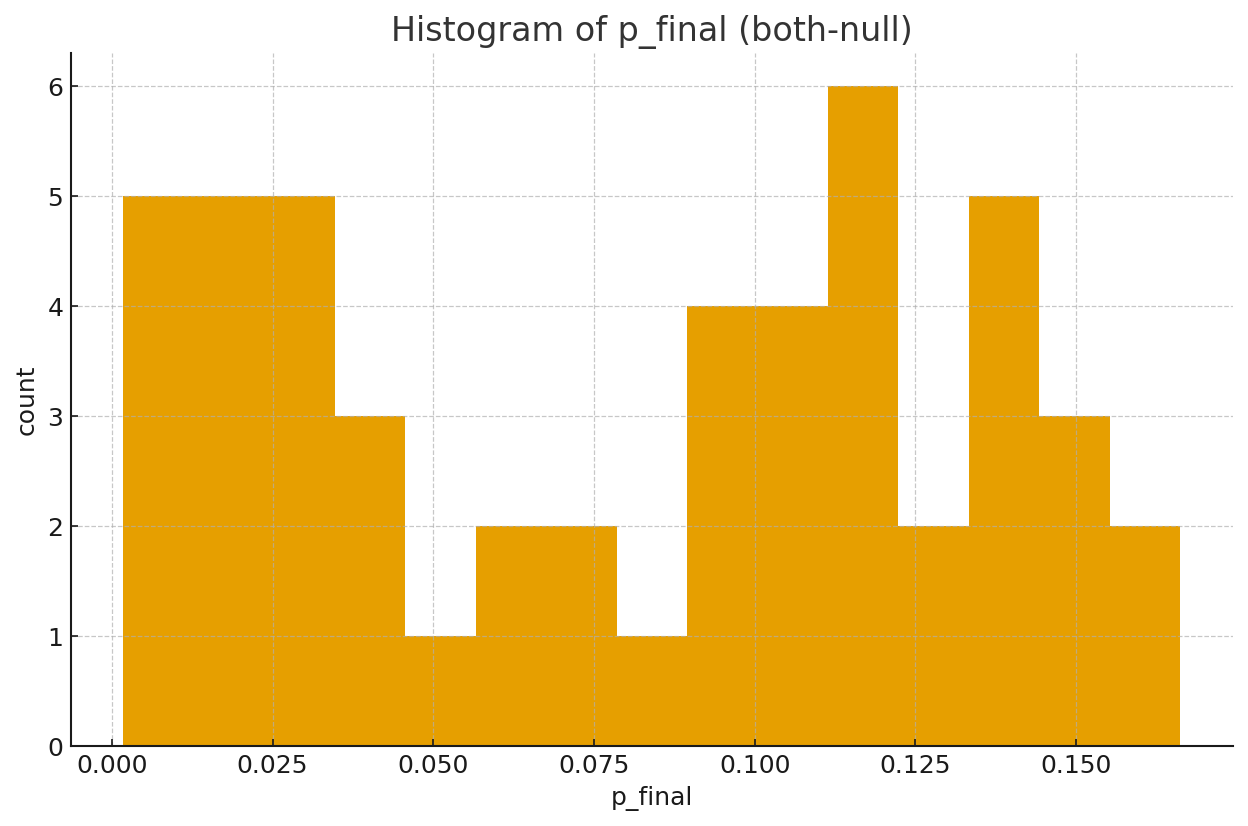
\includegraphics[width=0.72\linewidth]{figure/fig_T2_hist_both.png}
  \caption{Across 50 seeds under the conservative both-null, p_final is right-skewed with 18/50 < 0.05; min 0.0018, mean 0.08017.}
  \label{fig:T2-hist-both}
\end{figure}

\begin{figure}[ht]
  \centering
  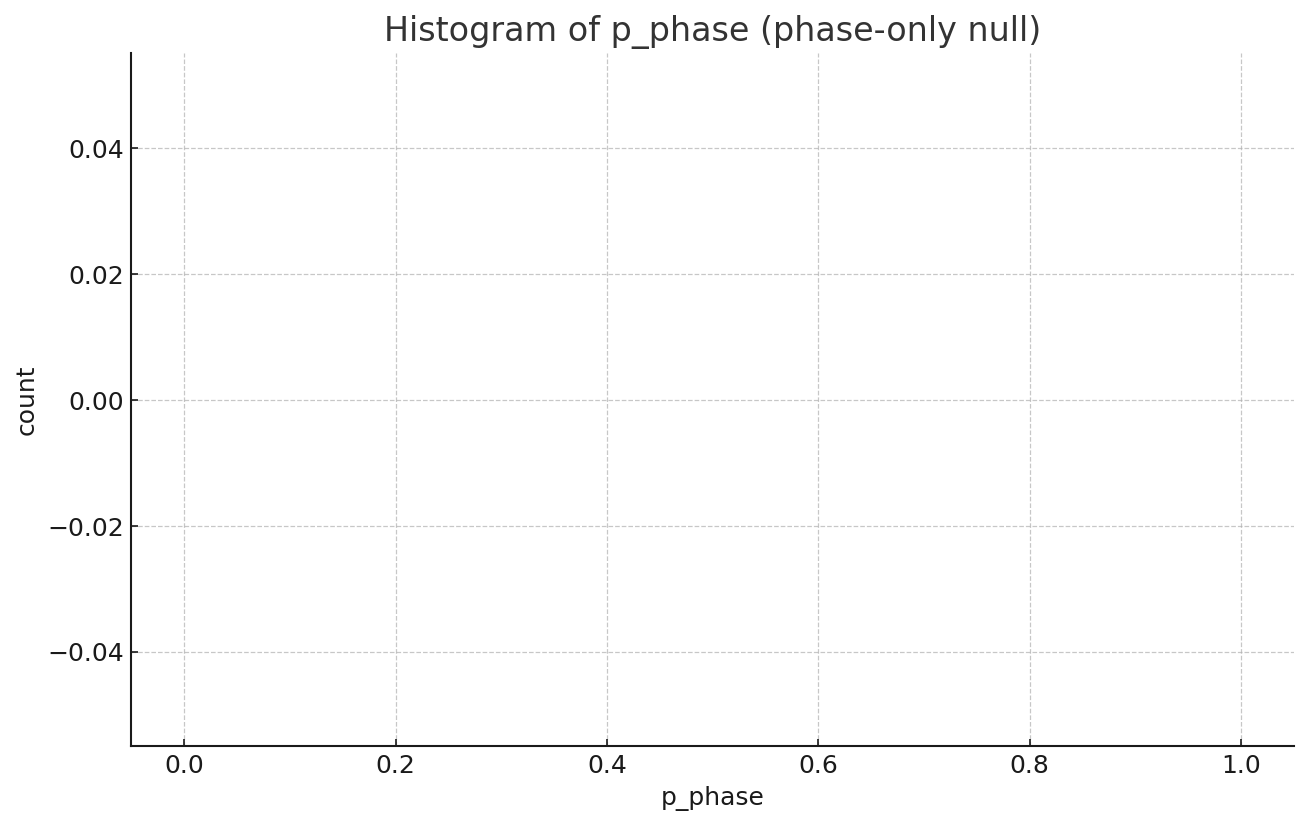
\includegraphics[width=0.72\linewidth]{figure/fig_T2_hist_phase.png}
  \caption{Phase-only surrogates are consistently rejected: 50/50 with p < 0.05; mean p ≈ 1.20e-05, max 0.0004.}
  \label{fig:T2-hist-phase}
\end{figure}

\begin{figure}[ht]
  \centering
  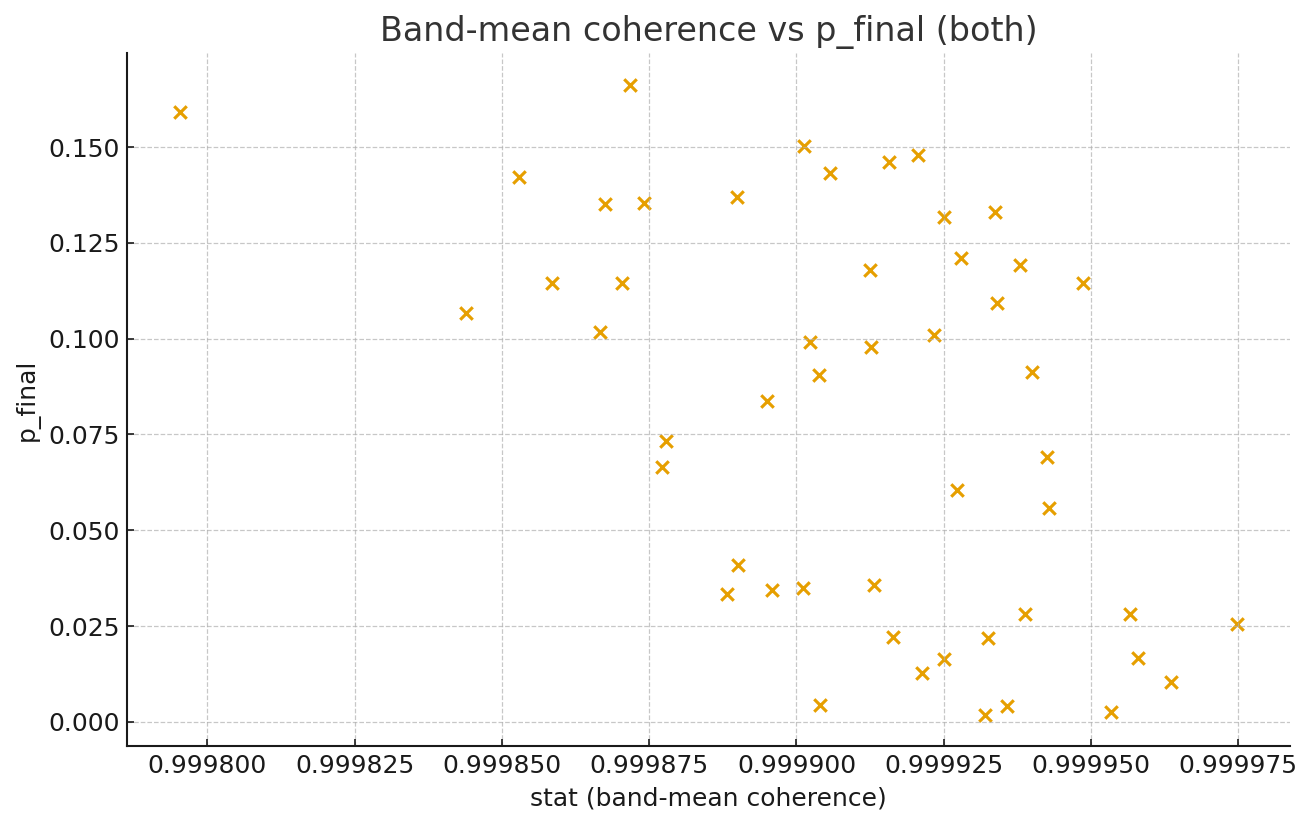
\includegraphics[width=0.72\linewidth]{figure/fig_T2_scatter_stat_vs_p.png}
  \caption{Higher band-mean coherence corresponds to lower p_final; best seeds fall below 0.01.}
  \label{fig:T2-scatter-stat-vs-p}
\end{figure}
% \input{figure/T3_figure_snippet.tex}

% Auto-generated T2 figures and captions (full 50-seed summary)
\begin{figure}[ht]
  \centering
  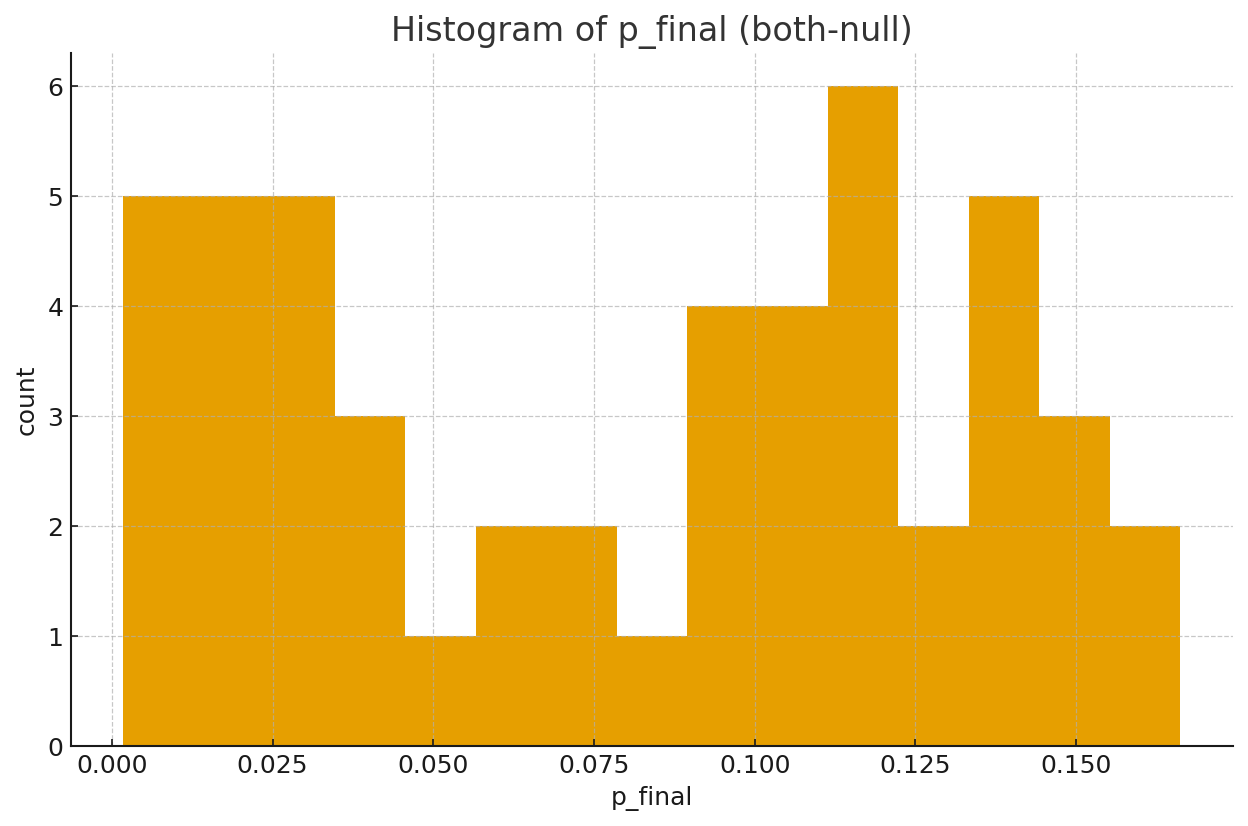
\includegraphics[width=0.72\linewidth]{figure/fig_T2_hist_both.png}
  \caption{Across 50 seeds under the conservative both-null, p_final is right-skewed with 18/50 < 0.05; min 0.0018, mean 0.08017.}
  \label{fig:T2-hist-both}
\end{figure}

\begin{figure}[ht]
  \centering
  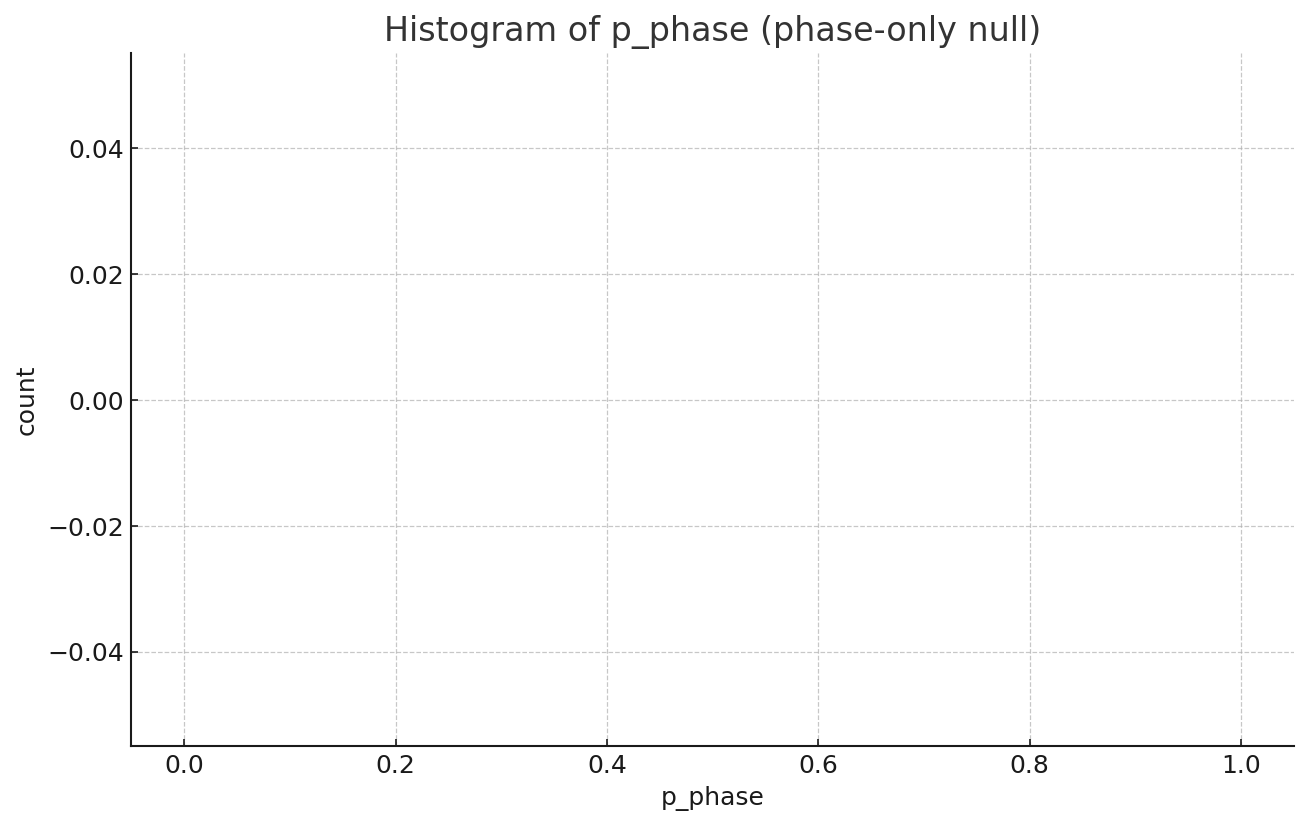
\includegraphics[width=0.72\linewidth]{figure/fig_T2_hist_phase.png}
  \caption{Phase-only surrogates are consistently rejected: 50/50 with p < 0.05; mean p ≈ 1.20e-05, max 0.0004.}
  \label{fig:T2-hist-phase}
\end{figure}

\begin{figure}[ht]
  \centering
  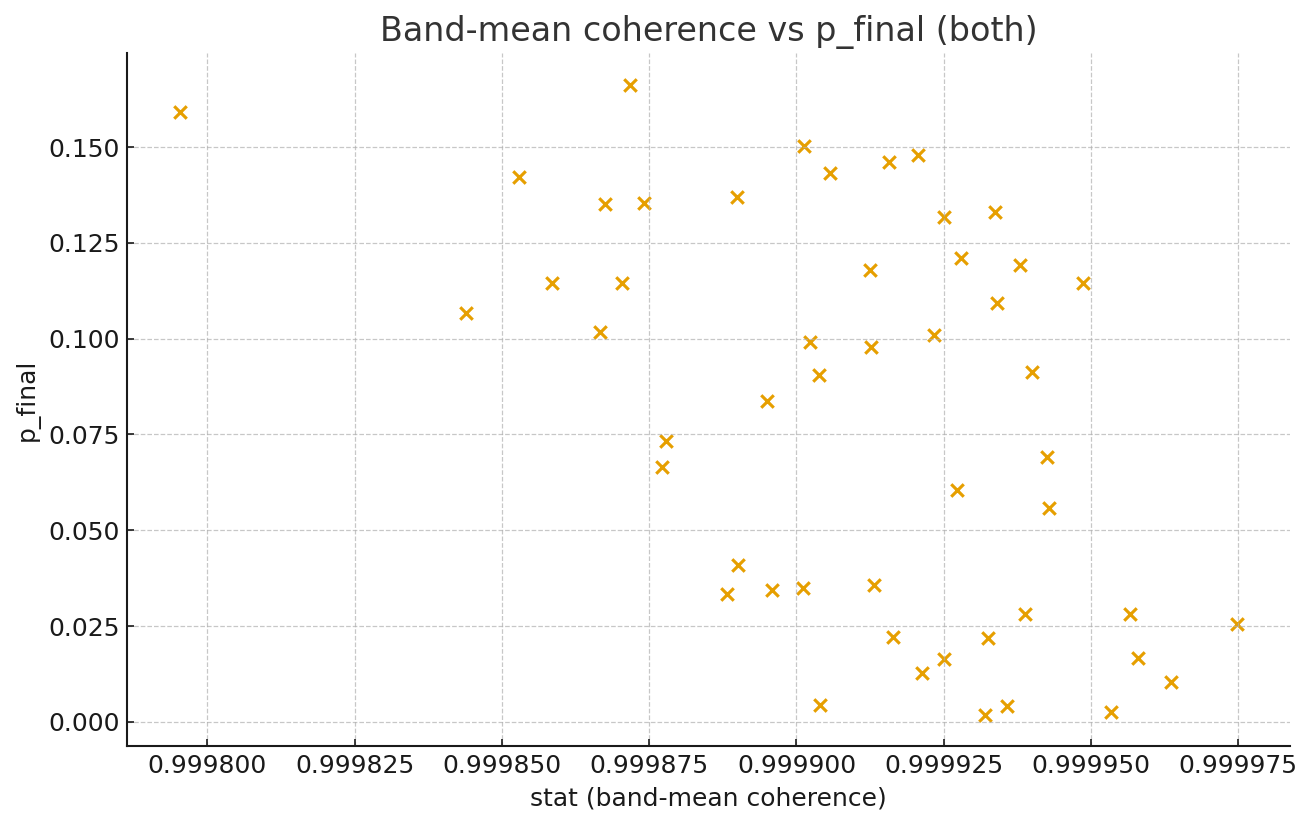
\includegraphics[width=0.72\linewidth]{figure/fig_T2_scatter_stat_vs_p.png}
  \caption{Higher band-mean coherence corresponds to lower p_final; best seeds fall below 0.01.}
  \label{fig:T2-scatter-stat-vs-p}
\end{figure}
\input{figure/T3_figure_snippet.tex}

% Optional tables with key metrics:
% \input{Tables_snippet.tex}

\section{Discussion}
% Interpretation, limitations, outlook.

\bibliographystyle{unsrt}
\bibliography{references}
\end{document}
